\documentclass[twocolumn,landscape,10pt]{article}
\usepackage[thinc]{esdiff} % for typesettign derivatives
\usepackage{amsthm} % provides an enhanced version of LaTex's \newtheorem command
\usepackage{mdframed} % framed environments that can split at page boundaries
\usepackage{enumitem} % bulletin points or other means of listing things
\usepackage{amssymb} % for AMS symbols
\usepackage{amsmath} % so as to use align
\usepackage{latexsym} % so as to use symbols like \leadsto
\usepackage{mathrsfs} % for using mathscr for char like operators
\usepackage{commath} % for using norm symbol
\usepackage{mathtools} % for using environments like dcases
\usepackage{authblk} % for writing affiliations
\usepackage{graphicx} % for importing images
\graphicspath{{./images/}} % for the path to images, also always put label behind captions
\usepackage{textcomp} % for using degree symbol
\usepackage{hyperref} % for clickable link in the pdf & customizable reference text
\usepackage[all]{hypcap} % for clickable link to images instead of caption
\usepackage[margin=1.0in]{geometry} % default is 1.5in
% \usepackage[left=0.4in, right=0.4in, top=0.8in, bottom=0.8in]{geometry}
\usepackage[title]{appendix} % for attaching appendix
\allowdisplaybreaks % allow page breaking in display maths, like align
\usepackage{xcolor} % for setting color of a block of text, use \textcolor{<color>}{}
\usepackage[normalem]{ulem} % for strikethrough text, use \sout{}
% allow for more advanced table layout
\usepackage{booktabs}
\usepackage{multirow}
\usepackage{siunitx}
% for adjusting caption settings
\usepackage{caption}
\captionsetup[table]{skip=10pt}

\theoremstyle{definition}
\mdfdefinestyle{defEnv}{%
  hidealllines=false,
  nobreak=true,
  innertopmargin=-1ex,
}

% The following is for writing block of code
\usepackage{listings}
\usepackage{color}

\definecolor{dkgreen}{rgb}{0,0.6,0}
\definecolor{gray}{rgb}{0.5,0.5,0.5}
\definecolor{mauve}{rgb}{0.58,0,0.82}

% setting of the thickness of the 4 lines of box
\setlength{\fboxrule}{2pt}

% Use the following to change code language and related settings
\lstset{frame=tb,
  language=Python,
  aboveskip=3mm,
  belowskip=3mm,
  showstringspaces=false,
  columns=flexible,
  basicstyle={\small\ttfamily},
  numbers=none,
  numberstyle=\tiny\color{gray},
  keywordstyle=\color{blue},
  commentstyle=\color{dkgreen},
  stringstyle=\color{mauve},
  breaklines=true,
  breakatwhitespace=true,
  tabsize=3,
  literate={~} {$\sim$}{1}
}

\pagestyle{headings}
\author{Lectured by Wenjia Bai}
\title{Computer Vision}
\affil{Typed by Aris Zhu Yi Qing}
\begin{document}
\maketitle
\tableofcontents

\newpage
\section{Image Filtering}

\subsection{Definition}

\begin{itemize}
    \item \underline{\textbf{Kernel}}: a small matrix used to apply effects,
        e.g. blurring.
    \item \underline{\textbf{Separable kernel}}: kernels that can be separated
        as two or more simple filters.
    \item \underline{\textbf{Padding}}: The action of adding pixels around the
        borders (e.g. with value 0) so that applying filters 
        will not reduce the size of the image.
    \item \underline{\textbf{Low-pass (smoothing) filter}}: filters that keep the
        low-frequency signals, e.g. MA filter
    \item \underline{\textbf{High-pass (sharpening) filter}}: filters that highlight the
        high-frequency signals, e.g. (identity + (identity - MA)) filter, or
        \[
            \begin{pmatrix}
                -\frac{1}{8} & -\frac{1}{8} & -\frac{1}{8} \\[4px]
                -\frac{1}{8} & 2 & -\frac{1}{8} \\[4px]
                -\frac{1}{8} & -\frac{1}{8} & -\frac{1}{8}
            \end{pmatrix}.
        \]
    \item \underline{\textbf{Denoising filter}}: filters to remove noise, e.g.
        median filter, non-local means, block-matching and 3D filtering (BM3D),
        etc.
\end{itemize} 


\subsection{Common Filters}

\subsubsection{Moving Average (MA) Filter}

\begin{itemize}
    \item In a 2D case, the MA kernel is a
        $\mathbb{R}^{K\times K}$ matrix in the following form
        \[
            \frac{1}{K^2}
            \begin{pmatrix}
                1 & 1 & \ldots & 1 \\
                1 & 1 & \ldots & 1 \\
                \vdots & \vdots & \ddots & \vdots \\
                1 & 1 & \ldots & 1
            \end{pmatrix} 
        \]
        with a time complexity of $O(N^2K^2)$, where $N$ is the legnth of image.
    \item MA kernel is separable, for instance
        \[
            \begin{pmatrix}
                \frac{1}{4} & \frac{1}{4} \\[4px]
                \frac{1}{4} & \frac{1}{4}
            \end{pmatrix} 
            =
            \begin{pmatrix}
                \frac{1}{2} & \frac{1}{2}
            \end{pmatrix} 
            *
            \begin{pmatrix}
                \frac{1}{2} \\[4px]
                \frac{1}{2}
            \end{pmatrix},
        \]
        reducing the time complexity to $O(N^2K)$.
    \item Purpose:
        \begin{itemize}
            \item remove high-frequency signal (noise or sharpness)
            \item result in a smooth but blurry image
        \end{itemize} 
\end{itemize} 

\subsubsection{Identity Filter}

The identity filter kernel is
\[
    \begin{pmatrix}
        0 & 0 & 0 \\
        0 & 1 & 0 \\
        0 & 0 & 0
    \end{pmatrix} 
\]

\subsubsection{Gaussian Filter}

\begin{itemize}
    \item The Gaussian kernel is a 2D Gaussian distribution
        \[
            h(i,j)=\frac{1}{2\pi\sigma^2}e^{-\frac{i^2+j^2}{2\sigma^2}}
        \]
        with $i,j=0$ as the centre of the kernel.
    \item While its support is infinite, small values outside
        $[-k\sigma,k\sigma]$ can be ignored, e.g. $k=3$ or $k=4$.
    \item 2D Gaussian filter is separable with
        \[
            h(i,j)=h_x(i) * h_y(j)
        \]
        where
        \[
            h_x(i)=\frac{1}{\sqrt{2\pi}\sigma}e^{-\frac{i^2}{2\sigma^2}},
        \]
        because
        \begin{align*}
            f[x,y]*h[x,y]
            & = \sum_i\sum_j f[x-i,y-j]h[i,j] \\
            & = \sum_i\sum_j
            f[x-i,y-j]\left(\frac{1}{2\pi\sigma^2}e^{-\frac{i^2+j^2}{2\sigma^2}}\right) \\
            & = \sum_i\left(\sum_j
            f[x-i,y-j]\frac{1}{\sqrt{2\pi}\sigma}e^{-\frac{j^2}{2\sigma^2}}\right)
            \frac{1}{\sqrt{2\pi}\sigma}e^{-\frac{i^2}{2\sigma^2}} \\
            & =
            \sum_i(f*h_y)[x-i]\frac{1}{\sqrt{2\pi}\sigam}e^{-\frac{i^2}{2\sigma^2}} \\
            & = (f*h_y)*h_x
        \end{align*} 
    \item Derivative of Gaussian filter $h$ is
        \[
            \frac{\mathrm{d}(f*h)}{\mathrm{d}x}=f*\frac{\mathrm{d}h}{\mathrm{d}x}
            =f*\frac{-x}{\sqrt{\pi}\sigma^3}e^{-\frac{x^2}{2\sigma^2}}.
        \]
        Thus, the smaller the $\sigma$, the more detail in the magnitude map;
        larger $\sigma$ suppresses noise and results in a smoother derivative.
        Different $\sigma$ help find edges at different scale.
\end{itemize} 

\subsubsection{Median Filter}

\begin{itemize}
    \item non-linear
    \item often used for denoising
    \item Move the sliding window, and replace the centre pixel using the median
        value in the window.
\end{itemize} 

\subsection{Impulse Response}

\begin{itemize}
    \item For continuous signal, an \underline{\textbf{impulse}} 
        is a Dirac delta function $\delta(x)$, with
        \[
            \delta(x)=
            \begin{cases}
                +\infty, & \text{if $x=0$} \\
                0, & \text{otherwise}
            \end{cases} 
        \]
        such that $\int_{-\infty}^{\infty} \delta(x)\mathrm{d}x=1$.
        For discrete signal, an impulse is a Kronecker delta function $\delta[i]$, with
        \[
            \delta[i]=
            \begin{cases}
                1, & \text{if $i=0$} \\
                0, & \text{otherwise}.
            \end{cases} 
        \]
    \item The \underline{\textbf{impulse response}} $h$ is the output of a filter
        when the input is an impulse. It completely characterises a
        \underline{\textbf{linear time-invariant}} filter.
        \begin{itemize}
            \item shifting the input signal $k$ steps corresponds to the same
                output signal but shifted by $k$ steps as well, e.g. assuming
                $f[n]=\delta[n]$, $g[n]=h[n]$,
                \begin{itemize}
                    \item $g[n]=10f[n]$ is time-invariant and amplifies the
                        input by a constant.
                    \item $g[n]=nf[n]$ is \emph{not} time-invariant since the
                        amount it amplies the input depends on the 
                \end{itemize} 
            \item if input $f_1[n]$ leads to $g_1[n]$, $f_2[n]$ leads to
                $g_2[n]$, we will have
                \[
                    \text{output}(\alpha f_1[n]+\beta f_2[n])=\alpha
                    g_1[n]+\beta g_2[n].
                \]
        \end{itemize} 
\end{itemize} 

\subsection{Convolution}

\begin{itemize}
    \item \underline{\textbf{Convolution}}: output $g$ can be described as the
        convolution between an input $f$ and impulse response $h$ as
        \[
            g[n]=f[n]*h[n]=
            \begin{dcases}
                \sum_{m=-\infty}^{\infty} f[m]h[n-m] & \text{discrete} \\
                \int_{m=-\infty}^{\infty} f(m)h(n-m) & \text{continuous} \\
            \end{dcases} 
        \]
    \item Note that if we describe input signal $f[n]$ as
        \[
            f[n]=\sum_{i=0}^{n} f[i]\delta[n-i]
        \]
        and we known the output of $\delta[n]$ is $h[n]$, we can write the
        output as
        \[
            g[n]=\sum_{i=0}^{n} f[i]h[n-i]
        \]
    \item commutative, i.e.\ 
        \[
            f[n]*h[n] = h[n]*f[n]
        \]
    \item associative, i.e.\
        \[
            f*(g*h)=(f*g)*h
        \]
    \item distributivity, i.e.\
        \[
            f*(g+h)=f*g+f*h
            \quad\text{and}\quad
            \frac{\mathrm{d}(f*g)}{\mathrm{d}x}=\frac{\mathrm{d}f}{\mathrm{d}x}*g=f*\frac{\mathrm{d}g}{\mathrm{d}x}
        \]
    \item In 2D discrete case for image filtering,
        \begin{align*}
            g[m,n]=f[m,n]*h[m,n]
            & =\sum_{i=-\infty}^{\infty}\sum_{j=-\infty}^{\infty}
            f[i,j]h[m-i,n-j] \\
            & =\sum_{i=-\infty}^{\infty}\sum_{j=-\infty}^{\infty}
            f[m-i,n-j]h[i,j]
        \end{align*} 
        if the dimension of the kernel is $(2M+1)\times(2N+1)$, we can write
        \[
            (f*h)[m,n]=\sum_{i=-M}^{M} \sum_{j=-N}^{N}
            f[m-i,n-j]h[i,j]
        \]
        with $h[0,0]$ being the centre of the filter, $(m,n)$ being the
        location in the image which the kernel's center is on.
    \item If a big filter $f_b$ can be separated into convolution $g$
        and $h$, we can first convolve with $g$, then $h$
        \[
            f*f_b=f*(g*h)=(f*g)*h.
        \]
\end{itemize} 

\section{Edge Detection}

\subsection{Detection}

\begin{table}[h]
    \centering
    \begin{tabular}{l|c|c}
          & finite difference & convolution kernel \\
        \hline
        Forward difference & $f'[x]=f[x+1]-f[x]$ & $[1,-1,0]$ \\
        \hline
        Backward difference & $f'[x]=f[x]-f[x-1]$ & $[0,1,-1]$ \\
        \hline
        Central difference & $f'[x]=(f[x+1]-f[x-1])/2$ & $[1,0,-1]$
    \end{tabular} 
\end{table} 

\subsection{Edge Detection Filters}

\subsubsection{Prewitt Filter}

Along the $x$-axis and the $y$-axis, we have respectively
\[
    \begin{pmatrix}
        1 & 0 & -1 \\
        1 & 0 & -1 \\
        1 & 0 & -1
    \end{pmatrix} 
    \quad\text{and}\quad
    \begin{pmatrix}
        1 & 1 & 1 \\
        0 & 0 & 0 \\
        -1 & -1 & -1
    \end{pmatrix}.
\]
They are separable, i.e.\
\[
    \begin{pmatrix}
        1 & 0 & -1 \\
        1 & 0 & -1 \\
        1 & 0 & -1
    \end{pmatrix} 
    =
    \begin{pmatrix}
        1 \\
        1 \\
        1
    \end{pmatrix} 
    *
    \begin{pmatrix}
        1 & 0 & -1
    \end{pmatrix}.
\]

\subsubsection{Sobel Filter}

Along the $x$-axis and the $y$-axis, we have respectively
\[
    \begin{pmatrix}
        1 & 0 & -1 \\
        2 & 0 & -2 \\
        1 & 0 & -1 \\
    \end{pmatrix} 
    \quad\text{and}\quad
    \begin{pmatrix}
        1 & 2 & 1 \\
        0 & 0 & 0 \\
        -1 & -2 & -1
    \end{pmatrix}.
\]
They are also separable, i.e.\
\[
    \begin{pmatrix}
        1 & 0 & -1 \\
        2 & 0 & -2 \\
        1 & 0 & -1 \\
    \end{pmatrix} 
    =
    \begin{pmatrix}
        1 \\
        2 \\ 
        1
    \end{pmatrix} 
    *
    \begin{pmatrix}
        -1 & 0 & -1
    \end{pmatrix} 
\]

\subsubsection{Magnitude and Orientation Calculation}

Let $h_x$ denotes the horizontal filter, $h_y$ denotes the vertical filter,
we can compute the magnitude and the orientation as
\begin{align*}
    g_x=f*h_x && \text{derivative along $x$-axis} \\
    g_y=f*h_y & &\text{derivative along $y$-axis} \\
    g = \sqrt{g_x^2+g_y^2} && \text{magnitude of the gradient} \\
    \theta = \text{arctan}{(g_y,g_x)} && \text{angle of the gradient}
\end{align*}

\subsection{Canny Edge Detection}

\subsubsection{Criteria for Good Edge Detector}

\begin{itemize}
    \item \underline{good detection}: low probability of FP/FN on marking edge points
    \item \underline{good localisation}: mark as close as the centre of true edge
    \item \underline{single response}: only one response to a single edge
\end{itemize} 

\subsubsection{Algorithm}

\begin{enumerate}
    \item perform Gaussian filtering to suppress noise
    \item calucalte the gradient magnitude $M(x,y)$ and direction
    \item apply Non-Maximum Suppression (NMS) to get a single response for each
        edge
        \[
            M(x,y)=
            \begin{cases}
                M(x,y) & \text{if local maximum} \\
                0 & \text{otherwise}
            \end{cases} 
        \]
    \item perform hyteresis thresholding to find potential edges with two
        thresholds $t_\text{low}$ and $t_\text{high}$\\
        \[
            \begin{cases}
                M(x,y) \ge t_\text{high} & \text{accept} \\
                M(x,y) < t_\text{low} & \text{reject} \\
                \text{Otherwise} & \text{\parbox[t]{6.5cm}{iteratively check neighbouring pixels 
                and accept if connected to an edge pixel.}}
            \end{cases} 
        \]
    \item evaluation/performance
        \begin{itemize}
            \item good detection --- FP reduced by Gaussian smoothing and FN
                reduced by hysteresis thresholding to find weak edges
            \item good localisation --- NMS finds locations based on gradient
                magnitude and direction
            \item single response --- NMS finds one single point in the
                neighbourhood
        \end{itemize} 
\end{enumerate} 


\section{Hough Transform}

\begin{itemize}
    \item \underline{\textbf{Hough transform}} is a transform from image space
        to parameter space, e.g. from an edge map to the two parameters of a
        line.
    \item output is a parametric model, given the input edge points
    \item each edge point vote for possible models in the parameter space
    \item Example:
        \begin{itemize}
            \item use slope intercept $b=y-mx$ to be the line model
            \item each edge point poll vote for different $b$ and $m$ values
                (also lines in parameter space)
            \item In practice, we use 2D bins to divide the parameter space;
                each point increases the vote by 1 in one of the bins,
                as shown in figure \ref{fig:hough_grid}.
                \begin{figure}
                  	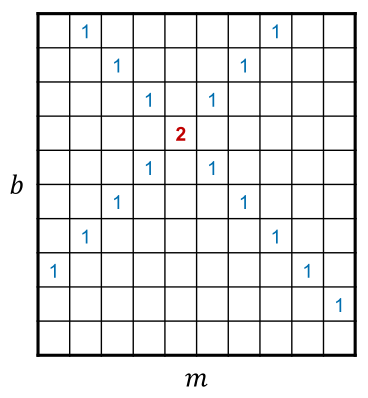
\includegraphics[scale=0.45]{hough_grid.png}
                  	\centering
                  	\caption{hough transform grid}\label{fig:hough_grid}
                \end{figure}
            \item But the parameter space could be too large,
                $[-\infty,+\infty]$; use \emph{normal
                form} instead
                \[
                    x\cos{\theta}+y\sin{\theta}=\rho
                \]
                so at least for one dimension, $\theta\in[0,\pi)$.
        \end{itemize} 
    \item Line detection by Hough transform:
        \begin{enumerate}
            \item Initialize the bins $H(\rho,\theta)$ to all zeros.
            \item For each $(x,y)$ and each $\theta$, calculate $\rho$ and
                $H(\rho,\theta)++$.
            \item Find $(\rho,\theta)$ where $H(\rho,\theta)$ is a local maximum
                and larger than a threshold.
                \begin{itemize}
                    \item local maximum so there can be multiple solutions, to
                        reduce FN
                    \item larger than a threshold so as to reduce FP
                \end{itemize} 
            \item The detected lines are given by
                $\rho=x\cos{\theta}+y\sin{\theta}$.
        \end{enumerate} 
    \item robust to noise/occlusion
        \begin{itemize}
            \item edge map is often generated after image smoothing
            \item broken/unoccluded edge points can still 
                vote and contribute to line detection
        \end{itemize} 
    \item Circle detection by Hough transform
        \begin{itemize}
            \item  parameter space also forms circles
            \item If radius $r$ is also unknown, then 3D parameter space
                $H(a,b,r)$
            \item parameterize to be $x = a+r\cos{\theta}$ and $y =
                b+r\sin{\theta}$, since we know $\theta$ form edge detection, we
                can narrow the voting area to move along $\theta$ for a distance
                $r$.
        \end{itemize} 
    \item Pros and Cons:
        \begin{itemize}
            \item[+] detects multiple instances
            \item[+] robust to image noise
            \item[+] robust to occlusion
            \item[-] Computational complexity is quite high. For each edge
                point, we need to vote to a 2D or even 3D parameter space.
            \item[-] need to carefully set parameters such as those for edge
                detectors, the threshold for the accumulator or range of circle
                radius.
        \end{itemize} 
\end{itemize} 


\section{Interest Point Detection}

\subsection{Definition}

\begin{itemize}
    \item \underline{\textbf{Interest point}}: points that we are interested in
        and are useful for subsequent image processing and analysis.
        They are also called \emph{keypoints}, \emph{landmarks},
        \emph{low-level} features.
\end{itemize} 

\subsection{Harris Detection}

\begin{itemize}
    \item small windows to tell if it is a corner
        \begin{itemize}
            \item flat --- change of intensity in neighter direction
            \item edge --- change of intensity along just one direction
            \item corner --- change of intensity along both direction
        \end{itemize} 
    \item If the window shifts by $[u,v]$, together with Taylor expansion
        \[
            I(x+u,y+v)=I(x,y)+uI_x(x,y)+vI_y(x,y)+\cdots
        \]the change of intensities is given by
        \begin{align*}
            E(u,v)
            &=\sum_{(x,y)\in W} w(x,y){[I(x+u,y+v)-I(x,y)]}^{2}\\
            &=\sum w(x,y){[uI_x(x,y)+vI_y(x,y)]}^{2}\\
            &=\sum w(x,y)(u^2I_x^2+2uvI_xI_y+v^2I_y^2)\\
            &=\sum w(x,y)
            \begin{pmatrix}
                u & v
            \end{pmatrix} 
            \begin{pmatrix}
                I_x^2 & I_xI_y \\
                I_xI_y & I_y^2
            \end{pmatrix} 
            \begin{pmatrix}
                u \\
                v
            \end{pmatrix} \\
            &=\begin{pmatrix}
                u & v
            \end{pmatrix} 
            \sum w(x,y)\begin{pmatrix}
                I_x^2 & I_xI_y \\
                I_xI_y & I_y^2
            \end{pmatrix} 
            \begin{pmatrix}
                u \\
                v
            \end{pmatrix} \\
            &:=\begin{pmatrix}
                u & v
            \end{pmatrix} 
            M
            \begin{pmatrix}
                u \\
                v
            \end{pmatrix}
        \end{align*} 
    \item $E$ is large if image derivatives are large
    \item We can infer the directions of change from $M$
        \begin{itemize}
            \item If $M=\begin{pmatrix}
                    0 & 0 \\
                    0 & 0
            \end{pmatrix} $,
            this is a \underline{\emph{flat}} region.
        \item If $M=\begin{pmatrix}
                10 & 0 \\
                0 & 0.1
            \end{pmatrix} $,
            large change if shift along $u$ $\Rightarrow$ an \underline{\emph{edge}}.
        \item If $M=\begin{pmatrix}
                10 & 0 \\
                0 & 10
            \end{pmatrix} $,
            large change in whichever way $\Rightarrow$ a \underline{\emph{corner}}.
        \item If more complicated $M$, we can do \underline{\textbf{eigen
            decomposition}} to obtain diagonal matrix $\Lambda$, and compare
            against the above 3 matrices.
        \end{itemize} 
    \item \underline{\textbf{Cornerness}} metrics:
        \begin{itemize}
            \item Harris and Stephens:
                \[
                    R = \lambda_1\lambda_2-k{(\lambda_1+\lambda_2)}^{2}
                    =\text{det}(M)-k{(\text{trace}(M))}^{2}
                \]
                where $k$ is a small number, $k=0.05$.
            \item Kanade and Tomasi:
                \[
                    R = \text{min}(\lambda_1,\lambda_2)
                \]
            \item Noble:
                \[
                    R = \frac{\lambda_1\lambda_2}{\lambda_1+\lambda_2+\epsilon}
                \]
        \end{itemize} 
    \item also detects blobs and textures
    \item algorithm:
        \begin{enumerate}
            \item compute $x$ and $y$ derivative of an image
                \[
                    I_x=G_x*I, I_y=G_y*I
                \]
                where $G$ can be e.g. sobel filter
            \item at each pixel, compute
                \[
                    M=\sum_{x,y}w(x,y)\begin{pmatrix}
                        I_x^2 & I_xI_y \\
                        I_xI_y & I_y^2
                    \end{pmatrix} 
                \]
            \item calculate detector response and detect interest point which
                are local maxima and whose $R$ is above threshold.
        \end{enumerate} 
    \item \underline{\emph{scaled}} Harrison detector:
        \[
            M = \sum_{x,y} w(x,y)\sigma^2
            \begin{pmatrix}
                I_x^2 & I_xI_y \\
                I_xI_y & I_y^2
            \end{pmatrix} 
        \]
        so that 
        \begin{itemize}
            \item at each scale $\sigma$, determine the scale which gives us the
                largest detector response
            \item prevent "the larger the scale, the smaller the derivative
                magnitude" problem
        \end{itemize} 
    \item Algorithm: perform orignal Harrison detector steps for each scale, and
        then determine the interest point.
\end{itemize} 

\subsection{Laplacian of Gaussian (LOG)}

\begin{itemize}
    \item First perform Gaussian smoothing, then Laplacian Operator, i.e.
        \[
            \Delta(f*h)=\frac{\partial^2(f*h)}{\partial x^2}+
            \frac{\partial^2(f*h)}{\partial y^2}=f*
            \left(\frac{\partial^2h}{\partial x^2}+\frac{\partial^2h}{\partial
            y^2}\right)
        \]
        where $h$ is the Gaussian kernel and $\Delta
        f=\frac{\partial^2f}{\partial x^2}+\frac{\partial^2f}{\partial y^2}$,
        with the following laplacian filter
        \[
            \begin{pmatrix}
                0 & 1 & 0 \\
                1 & -4 & 1 \\
                0 & 1 & 0
            \end{pmatrix} 
            =
            \begin{pmatrix}
                0 & 0 & 0 \\
                1 & -2 & 1 \\
                0 & 0 & 0
            \end{pmatrix} 
            +
            \begin{pmatrix}
                0 & 1 & 0 \\
                0 & -2 & 0 \\
                0 & 1 & 0
            \end{pmatrix} 
        \]
        Since we know the formation of a 2D Gaussian, we can derive the
        following:
        \[
            \frac{\partial^2h}{\partial x^2}+\frac{\partial^2h}{\partial y^2}
            =-\frac{1}{\pi\sigma^4}\left(1-\frac{x^2+y^2}{2\sigma^2}\right)
            e^{-\frac{x^2+y^2}{2\sigma^2}}
        \]
    \item To ensure comparability between scales, we do
        \[
            \text{LoG}_\text{norm}(x,y,\sigma)=\sigma^2(I_{xx}(x,y,\sigma)+I_{yy}(x,y,\sigma))
        \]
        similar to Harrison detector.
\end{itemize} 

\subsection{Difference of Gaussian (DoG)}

\begin{itemize}
    \item DoG is defined as\[
            \text{DoG}(x,y,\sigma):=I*G(k\sigma)-I*G(\sigma)
            \approx (k-1)\sigma^2\nabla^2G(x,y,\sigma)
        \]
        as an approximation of $\text{LoG}_\text{norm}$ using Gaussian filters
        at different scales.
    \item DoG filters are used in SIFT, which is a pipeline for detecting and
        describing interest points.
    \item ALso \underline{\textbf{scale-invariant}}, and follow similar
        procedures as above.
\end{itemize} 


\section{Feature Description}

\subsection{Simple Descriptors}

\begin{itemize}
    \item Pixel intensity
        \begin{itemize}
            \item[-] sensitive to absolute intensity value --- same object with
                different illumination can have different intensity
            \item[-] not very discriminative --- a single pixel doesn't
                represent any local content
        \end{itemize} 
    \item Patch intensities
        \begin{itemize}
            \item[+] respresent local pattern
            \item[+] perform well if the images are of similar intensities and roughly
                aligned
            \item[-] sensitive to absolute intensity value
            \item[-] not rotation-invariant
        \end{itemize} 
    \item Gradient orientation
        \begin{itemize}
            \item[+] sensitive to intensity changes
            \item[+] orientation is robust to scaling
            \item[-] not rotation-invariant
        \end{itemize} 
    \item Histogram
        \begin{itemize}
            \item[+] robust to rotation
            \item[+] robust to scaling
            \item[-] sensitive to intensity changes
        \end{itemize} 
\end{itemize} 

\subsection{Scale-Invariant Feature Transform (SIFT)}

\begin{itemize}
    \item detects and describe local features in images
    \item transforms an image into a large set of interest points, each of which
        is described by a feature vector that is \emph{\underline{invariant}} to
        \underline{translation}, \underline{scaling}, and \underline{rotation}.
    \item Algorithm:
        \begin{enumerate}
            \item detection of scale-space extrema (minima/maxima)

                search across scales and pixel locations, looking for interest
                points using DoG.

            \item keypoint localisation

                refine the estimate coordinates by fitting a quadratic curve to
                the neighbouring pixels and compute the new extrema.

                Denote the DoG response as $D(x,y,\sigma)$ or $D(\mathbf{x})$,
                by Taylor expansion we have
                \[
                    D(\mathbf{x}+\Delta \mathbf{x})=D(\mathbf{x})
                    +\frac{\partial D}{\partial \mathbf{x}}^T\Deta\mathbf{x}
                    +\frac{1}{2}\Delta\mathbf{x}\frac{\partial^2 D}{\partial
                    \mathbf{x}^2}\Delta\mathbf{x}
                \]
                \[
                    \Rightarrow
                    \frac{\partial
                    D(\mathbf{x}+\Delta\mathbf{x})}{\partial\Delta\mathbf{x}}
                    =\frac{\partial D}{\partial \mathbf{x}}
                    +\frac{\partial^2D}{\partial \mathbf{x}^2}\Delta\mathbf{x}
                    =0
                    \Rightarrow
                    \Delta\mathbf{x}=-{\left(\frac{\partial^2D}{\partial
                    \mathbf{x}^2}\right)}^{-1}\frac{\partial D}{\partial \mathbf{x}}
                \]

            \item orientation assignment

                determine the dominant orientation $\theta$ for a neighbourhood
                of a keypoint
                \begin{enumerate}
                    \item  an orientation histogram with 36 bins covering 360
                        degrees is created
                    \item each pixel votes for an orientation bin, weighted by
                        the gradient magnitude
                    \item keypoint will be assigned an orientation, which is the
                        peak of the historgram
                \end{enumerate} 
                So now we have the location $(x,y)$, scale $\sigma$, and
                dominant orientation $\theta$.

            \item keypoint descriptor
                
                Compute a histogram of gradient orientations. In practice,
                subregions are used and each subregion has 4x4 samples.
                \begin{itemize}
                    \item each subregions has one orientation histogram
                    \item these multiple histograms together describe what it
                        looks like around the keypoint.
                    \item each subregion has an orientation historgram with 8
                        bins in 8 directions.
                \end{itemize} 
                If 16 subregions are used, the descriptor (feature vector) 
                has a dimension of $128=16\times 8$.
        \end{enumerate} 
    \item robust to rotation, scaling, and changes in illumination
        \begin{itemize}
            \item rotation --- relative to dominant direction
            \item scaling --- draw samples from a window proportional to size
            \item changes in illumination --- using gradient orientations
        \end{itemize} 
\end{itemize} 

\subsection{Keypoint matching}

Suppose we find a keypoint $(x,y)$ in $A$ that corresponds to a keypoint $(u,v)$
in $B$. We assume that they are reltaed with an \emph{affine} transformation:
\[
    \begin{pmatrix}
        u \\
        v
    \end{pmatrix} 
    =
    \begin{pmatrix}
        m_1 & m_2 \\
        m_3 & m_4
    \end{pmatrix} 
    \begin{pmatrix}
        x \\
        y
    \end{pmatrix} 
    +
    \begin{pmatrix}
        t_x \\
        t_y
    \end{pmatrix} 
\]
with many pairs of corresponding keypoints, we can write the equation as:
\[
    \begin{pmatrix}
        x_1 & y_1 & 0 & 0 & 1 & 0 \\
        0 & 0 & x_1 & y_1 & 0 & 1 \\
        x_2 & y_2 & 0 & 0 & 1 & 0 \\
        0 & 0 & x_2 & y_2 & 0 & 1 \\
        \vdots & \vdots & \vdots & \vdots & \vdots & \vdots
    \end{pmatrix} 
    \begin{pmatrix}
        m_1 \\
        m_2 \\
        m_3 \\
        m_4 \\
        t_x \\
        t_y
    \end{pmatrix} 
    =
    \begin{pmatrix}
        u_1 \\
        v_1 \\
        u_2 \\
        v_2 \\
        \vdots
    \end{pmatrix} 
\]
which can be written as a linear system
\[
    A\mathbf{m}=\mathbf{b}
\]where only $\mathbf{m}$ is unknown, and solve the least-square problem as
\[
    \mathbf{m}={(A^TA)}^{-1}A^T\mathbf{b}
\]

\subsection{RANSAC}

However, the squared difference, $\norm{A\mathbf{m}-\mathbf{b}}^2$, can be sensitive to
outliers(noise) --- points that are deemed to be corresponding but actually
aren't. To ensure the robustness to outliers. RANSAC(Random Sample Consensus) deals with this.
\begin{enumerate}
    \item randomly sample some points
    \item fit a line along the sampled points
    \item find the number of \underline{\textbf{inliers}} within a threshold to
        the line
    \item terminate if enough inliers have been found, or we have reached a
        certain number of iteration
\end{enumerate} 

\subsection{Acceleration}

\subsubsection{Speeded-Up Robust Features (SURF)}

\begin{itemize}
    \item SURF only computes the gradients along horizontal and vertical
        directions using \underline{\textbf{Haar wavelets}}.
    \item SURF applies very simple filters $d_x$ and $d_y$
        \[
            d_x=
            \begin{pmatrix}
                -\mathbf{1} & \mathbf{1}
            \end{pmatrix},
            d_y=
            \begin{pmatrix}
                -\mathbf{1}^T \\
                \mathbf{1}^T
            \end{pmatrix} 
        \]
        where $\mathbf{1}^T=\begin{pmatrix}
            1 & 1 & \ldots & 1
        \end{pmatrix} $ called the Haar wavelets
    \item Summing pixel intensities with weigths 1 and -1 is very fast, so the
        result for each subregion is defined by (the sum of values and the sum
        of absolute values)
        \[
            \left(\sum d_x,\sum d_y, \sum|d_x|,\sum|d_y|\right)
        \]
        \begin{itemize}
            \item all four are low --- homogeneous subregion
            \item zebra pattern/strips --- $\sum|d_x|$ or $\sum|d_y|$ is high
            \item gradually increasing intensities --- $\sum|d_x|$ and $\sum d_x$ are
                high
        \end{itemize} 
    \item Now we need $16\times 4 = 64 $ dimensions, and around 5 times faster
        than SIFT with Haar wavelets.
\end{itemize} 

\subsubsection{Binary Robust Independent Elementary Features (BRIEF)}

\begin{itemize}
    \item we compare an interest point $p$ to another interest point $q$
        and get a binary value as output
        \[
            \tau(p,q)=
            \begin{cases}
                1 & \text{if }I(p)<I(q) \\
                0 & \text{otherwise}.
            \end{cases} 
        \]
    \item randomly sample $n_d$ pairs of points for binary tests; random pattern
        is only determined once and same pattern applied to all intersect
        points.
        \begin{itemize}
            \item If $n_d=256$, we have 256 tests in total, with a total of 32
                bytes (SURF uses 64 bytes).
            \item fast to compute with bit-shifting operator \texttt{<<} and
                \texttt{>>}.
            \item use bitwise XOR between two descriptors to get the
                \underline{\textbf{hamming distance}} instead of Euclidean
                distance, which is the bit count of the result.
        \end{itemize} 
    \item ignores rotation and scaling, assume images are taken from a moving
        camera with only translation.
    \item about 40-fold faster than SURF, which is around 200 times faster than
        SIFT.
\end{itemize} 

\subsubsection{Histograms of Oriented Gradient(HOG)}

\begin{itemize}
    \item we can extend the idea of feature descriptors to describe the feature
        of a large region, even a whole image.
    \item HOG divides a large region into a (dense) grid of cells, describes
        each cell, and concatenates the local descriptions to form a global
        description.
    \item The description vector $\mathbf{v}$ for each cell is normalized to form a
        locally normalized descriptor as
        \[
            \mathbf{v}_\text{norm}=\frac{\mathbf{v}}{\sqrt{\norm{\mathbf{v}}^2_2+\epsilon^2}}
        \]
        with $\epsilon$ to ensure numerical stability
\end{itemize} 


\section{Image Classification}

\subsection{Classification concepts}

See Intro to ML notes for $k$-NN, distance metrics, parameter tuning,
cross-validation, stachastic gradient descent, multi-layer perceptron,
forward/backward propagation


\subsection{Support Vector Machine (SVN)}

\begin{itemize}
    \item If used as a \emph{linear} SVN, the model is formulated as
        \[
            \mathbf{w}\cdot\mathbf{x}+b=0
        \]
        The rule is to assign a class $c$ to data $x$ with
        \[
            c=
            \begin{cases}
                1 & \text{if }\mathbf{w}\cdot\mathbf{x}+b\ge 0 \\
                -1 & \text{otherwise}
            \end{cases} 
        \]
        so we need to estimate $\mathbf{w}$ and $b$ to determine the decision
        boudnary or \emph{hyperplane}.
    \item The problem could be transformed to an optimisation problem of
        \[
            \underset{\mathbf{w},b}{\text{min}}\norm{\mathbf{w}}^2
        \]
        subject to $y_i(\mathbf{w}\cdot \mathbf{x}_i+b)\ge 1$ for $i=1,2,\ldots,N$.
        Or formulate as
        \[
            \underset{\mathbf{w},b}{\text{min}}\norm{\mathbf{w}}^2
            +C\sum_{i=1}^{N} \max{(0,1-y_i(\mathbf{w}\cdot \mathbf{x}_i+b))}
        \]
        since we cannot guarantee the data to be linearly separable.
        The second term of the above is equation is called the
        \underline{\textbf{hinge loss}}.
        The gradient of the loss function is
        \[
            \nabla_\mathbf{w}L=2\mathbf{w}-C\sum_{i=1}^{N}\nabla_\mathbf{w}h
        \]
        where
        \[
            \nabla_\mathbf{w}h=
            \begin{cases}
                -y_i\mathbf{x}_i & \text{if }y_i(\mathbf{w}\cdot\mathbf{x}_i+b < 1) \\
                0 & \text{otherwise}
            \end{cases} 
        \]
        so at each iteration,
        \[
            \mathbf{w}^{(k+1)}=\mathbf{w}^{(k)}-\eta\nabla_\mathbf{w}L(\mathbf{w}^{(k)},b^{(k)})
        \]
\end{itemize} 

\subsection{Convolutional Neural Network}

\begin{itemize}
    \item In CNN, each neuron only see a small local region in the layer before
        it, called the \underline{\textbf{receptive field}}.
    \item e.g. A neuron can depend on a 5x5x$C$ cube of the input, where $C$
        refers to the number of color channels.
    \item More output neurons can be added as well, to form a $D$x1x1 cube,
        where $D$ denotes depth.
    \item Mathematically, a \underline{\textbf{convolution layer}} is
        \[
            a_d=f\left(\sum_{ijk}W_{dijk}x_{ijk}+b_d\right)
        \]
        where $d$ is the depth of output, $ij$ is the dimension coordinate, and
        $k$ is the input channel/depth.
    \item operations during convolution:
        \begin{itemize}
            \item \underline{\textbf{padding}}
            \item \underline{\textbf{stride}}
            \item \underline{\textbf{dilation}}: make a neuron look at a larger
                region (increase receptive field) by downsample image or increase kernel size
        \end{itemize} 
    \item \underline{\textbf{Pooling layer}}:
        \begin{itemize}
            \item operation to make feature maps/representations smaller
            \item similar to image downsampling, e.g. if max pooling, 
                \[
                    \begin{pmatrix}
                        1 & 2 \\
                        5 & 6
                    \end{pmatrix} 
                    \Rightarrow
                    \begin{pmatrix}
                        6
                    \end{pmatrix} 
                \]
                pick the max element, and reduce the dimension
        \end{itemize} 
    \item issue:
        \begin{itemize}
            \item  \emph{exploding} gradient --- clip it, such as clip by value
                \[
                    \mathbf{g}_i=
                    \begin{cases}
                        v_\text{min} & \text{if }g_i<v_\text{min} \\
                        v_\text{max} & \text{if }g_i>v_\text{max} \\
                        \mathbf{g}_i & \text{otherwise}
                    \end{cases} 
                \]
                or clip by norm
                \[
                    \mathbf{g}=
                    \begin{dcases}
                        \frac{\mathbf{g}}{\norm{\mathbf{g}}}v & \text{if }
                        \norm{\mathbf{g}}>v \\
                        \mathbf{g} & \text{otherwise}
                    \end{dcases} 
                \]
            \item \emph{vanishing} gradient --- use different activation
                functions, e.g. ReLU, leaky RelU, or
                \begin{itemize}
                    \item Parametric ReLU
                        \[
                            f(z)=
                            \begin{cases}
                                az & z < 0 \\
                                z & z \ge 0
                            \end{cases} 
                        \]
                    \item Exponential Linear Unit
                        \[
                            f(z)=
                            \begin{cases}
                                a(e^z-1) & z < 0 \\
                                z & z \ge 0
                            \end{cases} 
                        \]
                \end{itemize} 
        \end{itemize}
    \item Representative CNN: LeNet, AlexNet, VGG
\end{itemize} 

\section{Object Detection}

\subsection{Approaches}

\begin{itemize}
    \item general ideas
        \begin{itemize}
            \item at each sliding window, perform two tasks.
            \item Firstly, classification (whether this is a cat or not)
            \item secondly, localisation (bounding box coordinates) using CNN to
                predict bounding coordinates
            \item however, too expensive to apply CNN on each pixel of the image
        \end{itemize} 
    \item two-stage detection:
        \begin{enumrate}
            \item make an initial guess, propose some possible regions of
                interest
            \item classify what these regions are and predict the bounding boxes
        \end{enumrate} 
    \item One-stage detection:
        \begin{itemize}
            \item do not guess, but simply divide the image into grid cells
            \item classify these grid cells and predict the bounding boxes
        \end{itemize} 
\end{itemize} 

\subsection{Two-stage Object Detection Methods}

\subsubsection{Selective Search}

We can look at image features such as greyscale or gradients to separate the
image into regions with similar features.

\subsubsection{Faster R-CNN}

\subsubsubsection{\textbf{RPN}}

\begin{itemize}
    \item A \underline{\textbf{Region Proposal Network}} (RPN) is used.
    \item The input image is fed into a CNN, gives the image's feature map.
    \item The feature map goes into a RPN, outputing interesting regions to be
        looked at.
    \item Using AlexNet/VGG-16 as \underline{\textbf{backbone networks}}, using
        their last convolution layer as a feature map, we can use a $3\times 3$
        sliding window to perform binary classification at each location,
        giving it 0 if it isn't interesting, and 1 if it is.
    \item it handles objects of different sizes / aspect ratio by making $k$
        predictions(bounding boxes). e.g. $128^2$, $256^2$, $512^2$, $1:1$,
        $1:2$, $2:1$. These bounding boxes are called
        \underline{\textbf{anchors}}.
    \item A bounding box can be described by its centre coordinates $(x,y)$ and
        size $(w,h)$.
    \item For a convolution feature map of $W\times H$, $W\times H \times k$
        anchors are predicted, and only the highest scoring boxes are kept.
    \item The loss is defined as
        \[
            L(p,t) = \underbrace {\sum_{i=1}^{n_\text{anchor}} 
            L_\text{cls}(p_i,p_i^*)}_{\text{classification loss}} +
            \underbrace{\lambda\sum_{i=1}^{n_\text{anchor}}
            1_{y=1}L_\text{loc}(t_i,t_i^*)}_{\text{localisation loss}}
        \]
        where $^*$ denotes the ground truth
    \item we predict how to transform this anchor into the ground truth bounding
        box using:
        \begin{align*}
            \text{anchor} & = (x_a, y_a, w_a, h_a) \\
            \text{predicted bounding box} & = (x,y,w,h) \\
            \text{predicted transformation} & = (t_x,t_y,t_w,t_h) \\
            t_x & = \frac{x-x_a}{w_a} \\
            t_y & = \frac{y-y_a}{h_a} \\
            t_w & = \log{\frac{w}{w_a}} \\
            t_h & = \log{\frac{h}{h_a}}
        \end{align*} 
\end{itemize} 

\subsubsubsection{\textbf{RoI}}

\begin{itemize}
    \item Combining classification and localisation, we have features for each
        region known as \underline{\textbf{RoI}} (Region of Interest). We can
        use an RoI pooling layer, which we can calculate RoI location and size
        on the feature map and convert to a fixed size to be provided to the
        classifier.
    \item For each RoI, the classifier predicts the label class and refines the
        bounding box estimate:
        \[
            L(p,t)=L_\text{cls}(p,y)+\lambda\cdot 1_{y\ge 0}L_\text{loc}(t,t^*)
        \]
        where $y$ denotes the ground truth, and is now a multi-class
        classification problems.
\end{itemize} 

\subsubsubsection{\textbf{Comparison between RPN and Detection Network}}

Please see table \ref{table:rpn-roi}.

\begin{table}[h]
    \centering
    \caption{RPN v.s. RoI}
    \label{table:rpn-roi}
    \begin{tabular}{c|c}
        RPN & Detection network \\
        \hline \hline
        \rule{0mm}{12mm}
        \shortstack{The input to RPN is a $3\times 3$ \\
            window on conv5 feature map.} &
        \shortstack{The input to detection network \\is a proposed region, thus 
            \\contains more accurate features.} \\
        \hline
        \rule{0mm}{8mm}
        \shortstack{It is class-agnostic. It only checks \\
            whether this is an RoI or not.} &
        \shortstack{It classifies the region \\into a number of classes.} \\
        \hline
        \rule{0mm}{12mm}
        \shortstack{RPN needs to use a lot of anchors, \\
            because we do not know what \\
            the object looks like yet} & 
        \shortstack{It does not need to use anchors.\\
        We already know a rough size \\from the proposal.}
    \end{tabular} 
\end{table} 

\subsection{One-stage Object Detection Methods}

\begin{itemize}
    \item e.g. YOLO, SSD. The RPN is changed from using a binary value for the
        classification loss to using a multi-class classifier, which predicts the object
        for each anchor.
    \item Faster R-CNN is more accurate but slower, and vice versa for SSD,
        since RPN estimates the regions size before looking closely at features
        and then refining it.
    \item Backbone networks (VGG/AlexNet) can be changed out to improve
        performance.
\end{itemize} 

\section{Image Segmentation}

\subsection{Thresholding}

This converts a greyscale image to a binary label map. At each pixel, the label
is defined as
\[
    f(x)=
    \begin{cases}
        1 & \text{if }I(x)\ge \text{threshold} \\
        0 & \text{otherwise}.
    \end{cases} 
\]
This  doesn't require any training data, and only needs threshold as the
parameter.

\subsection{$K$-means}

\begin{itemize}
    \item unsupervised method
    \item Represents each cluster by its centre.
        Each data point (pixel intensity) is associated to the nearest cluster
        centre.
    \item It can be formulated as
        \begin{equation}\label{eq:KNN}
            \text{min}\sum_{k=1}^{K} \sum_{x\in C_k}{(x-\mu_k)}^{2}
            \quad\text{or}\quad
            \text{min}\sum_{k=1}^{K} \sum_{x}\delta_{x,k}{(x-\mu_k)}^{2}
        \end{equation} 
        where $\delta_{x,k}$ denotes membership of $x$ in cluster $k$, $\mu_k$
        denotes the centre of cluster $k$.
    \item Algorithm
        \begin{enumerate}
            \item initialize $\mu_k$, where $k=1,2,\ldots,K$.
            \item For each iteration
                \begin{enumerate}
                    \item  compute $\delta_{x,k}$ for each data point, assigning
                        $x$ to the nearest cluster centre $\mu_k$.
                    \item update $\mu_k$ according to the membership
                        $\delta_{x,k}$.
                    \item repeat until $\delta_{x,k}$ no longer changes or the
                        maximum number of iterations is reached.
                \end{enumerate} 
        \end{enumerate} 
    \item To determine which $K$ to use, plot equation \eqref{eq:KNN} with
        different $K$, and use the ``elbow'' method to determine the best value.
    \item clustering can also be performed base on
        \begin{itemize}
            \item color similarity
            \item position + color similarity
            \item other features
        \end{itemize} 
        so that $x$ becomes a feature vector instead of a scalar.
\end{itemize} 

\subsection{Gaussian Mixture Model (GMM)}

\begin{itemize}
    \item unsupervised method
    \item GMM performs a \emph{soft} assignment by assuming a Gaussian
        distribution for each cluster, formulated as
        \[
            P(y_j=k|x_j,\pi_k,\mu_k,\sigma_k)=
            \pi_k\cdot \frac{1}{\sqrt{2\pi}\sigma_k}
            e^{-\frac{{(x-\mu_k)}^{2}}{2\sigma^2_k}}
        \]
        where $x_j$ is the intensity of feature for data point $j$,
        $\pi_k$ is the mixing component for class $k$, $y_j$ denotes the group
        which point $j$ belongs to.
    \item See intro to ML for detailed algorithm.
\end{itemize} 

\subsection{CNN}

\begin{itemize}
    \item supervised method
    \item we can e.g. remove the fully connected layers and
        directly infer pixel-wise classification results 
        from the $13\times 13$ feature map
    \item \underline{\textbf{Fully convolutional network}}: all layers are
        convolutional layers.
    \item \underline{\textbf{Convolutionalization}}: replaces the fully
        connected layers with convolutional layers
    \item Need to apply \underline{\textbf{upsampling}} operation to obtain a
        pixel-wise prediction
        \begin{itemize}
            \item e.g. transposed convolution. 
                For $\mathbb{R}^{4\times 4}\mapsto\mathbb{R}^{8\times 8}$,
                we can have one input correspond to a $3\times 3$ region in the
                output, with some weight, with a stride of 2.
            \item convolution in 1D as matrix operation v.s. 2D, see figure
                \ref{fig:conv1d}.
                \begin{figure}[h]
                  	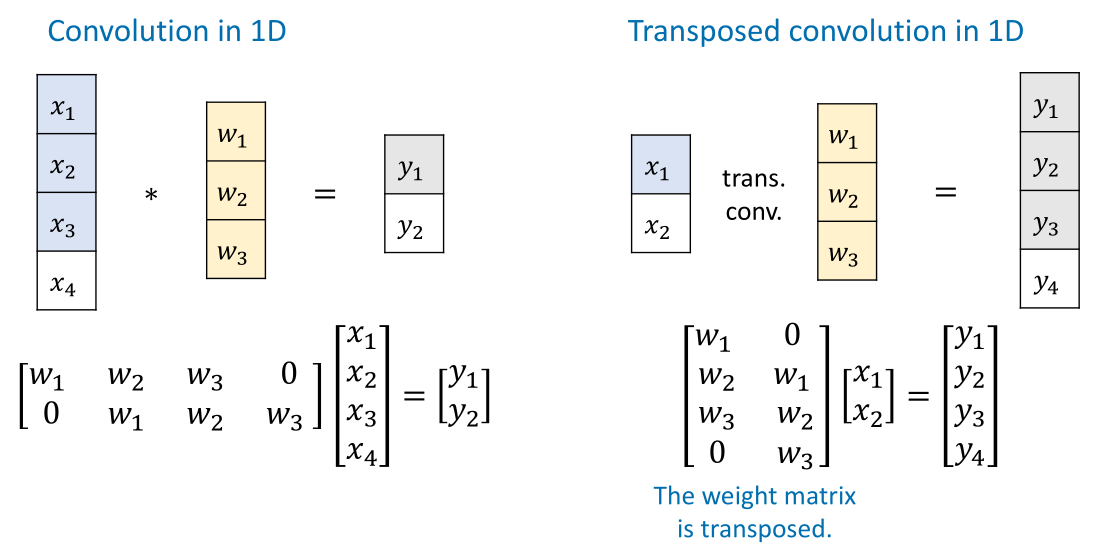
\includegraphics[scale=0.29]{1d-convolution.png}
                  	\centering
                  	\caption{convolution v.s. transposed convolution in Matrix
                    operation}\label{fig:conv1d}
                \end{figure}
                
        \end{itemize} 
    \item Thus a classification network can be transformed to a segmentation
        network by replacing the fully connected layers with convolutional and
        transposed convolutional layers.
    \item \underline{\textbf{Mask R-CNN}}
        \begin{itemize}
            \item the input is the convlution feature map
            \item fed into two branches: detection and segmentation
            \item segmentation branch is fully convolutional
        \end{itemize} 
\end{itemize} 




\end{document}
